%% Prob-Adaptive Inf-TESLA++ -- conference manuscript (IEEEtran).
%% No local LaTeX toolchain was available; compile on Overleaf or with a
%% standard TeX Live install: pdflatex -> bibtex (none needed, refs inline) -> pdflatex x2.
\documentclass[conference]{IEEEtran}
\IEEEoverridecommandlockouts
\usepackage{cite}
\usepackage{amsmath,amssymb,amsfonts}
\usepackage{algorithm}
\usepackage{algpseudocode}
\usepackage{graphicx}
\usepackage{booktabs}
\usepackage{textcomp}
\usepackage{xcolor}
\usepackage{url}
\def\BibTeX{{\rm B\kern-.05em{\sc i\kern-.025em b}\kern-.08emT\kern-.1667em\lower.7ex\hbox{E}\kern-.125emX}}

\begin{document}

\title{Prob-Adaptive Inf-TESLA++: Closed-Loop Slot-Duration Control for\\
Overflow-Resilient Broadcast Authentication on Constrained Radios}

\author{\IEEEauthorblockN{[Author Names]}
\IEEEauthorblockA{[Department / Institution]\\
[City, Country]\\
[emails]}}

\maketitle

\begin{abstract}
Time-delayed key disclosure (the TESLA family) authenticates broadcast traffic
without per-receiver state, and recent blockchain-anchored variants remove the
sender--receiver resynchronization step by committing hash-chain roots to a
smart contract. These protocols nonetheless run the disclosure schedule on a
\emph{fixed} slot timer. When a resource-constrained device (RCD) must push
authentication evidence through a slow or congested radio, the disclosure
pipeline fills faster than it drains; on overflow the evidence for a slot is
lost permanently and every message in that slot becomes unauthenticatable. We
present Prob-Adaptive Inf-TESLA++, a backward-compatible extension that replaces
the fixed slot timer with a closed-loop controller. At each slot boundary the
sender samples the pending-disclosure backlog, normalizes it to a target
utilization, and nudges the next slot duration up or down with a bounded
proportional (EIP-1559-style) rule, clamped to immutable on-chain bounds
$[T_{\min},T_{\max}]$. Longer slots batch more messages per disclosure and lower
the disclosure rate, letting the radio drain the backlog; shorter slots restore
low latency once pressure clears. We implement the extension on top of an
Inf-TESLA++ codebase in Go with a Solidity contract, and evaluate it end-to-end
against a live local blockchain by sweeping the authentication-channel radio
budget. The measured controller tracks the bottleneck: the slot duration rises
from its 1000\,ms floor to its 8000\,ms ceiling as the budget tightens, the
disclosure backlog stays bounded across a wide operating range, and
authentication remains alive down to a hard budget floor below which no slot
length can save it. We report the controller's characteristic curves,
quantify the stability boundary, and discuss the limitations of the prototype.
\end{abstract}

\begin{IEEEkeywords}
broadcast authentication, TESLA, delayed key disclosure, congestion control,
smart contracts, resource-constrained devices, IoT.
\end{IEEEkeywords}

\section{Introduction}
Broadcasting to many receivers at once is the natural communication pattern for
sensor fields, drone swarms, vehicular safety messages, and industrial
telemetry. Securing such traffic requires \emph{source authentication} that
scales to an unbounded, possibly unknown, receiver set without giving every
receiver the power to forge messages. Public-key signatures provide this but are
expensive for a device with a small CPU and a tight energy budget, and a
signature per packet is often unaffordable on the air interface.

The TESLA family~\cite{tesla} solves the problem with symmetric primitives and a
single asymmetry: \emph{time}. The sender commits to a reversed hash chain and
authenticates the messages of a time slot with a key that it reveals only after
a delay of $d$ slots. A receiver buffers the messages, waits for the delayed
key, checks that the key belongs to the committed chain, and verifies the
message authentication code. Because the key is disclosed only after the window
in which a forgery would be useful, an attacker who learns it can no longer
inject traffic for that slot. The scheme needs only loose time synchronization
and one hash-chain commitment per sender.

A practical obstacle to \emph{continuous} operation is that a finite hash chain
eventually runs out, and re-establishing a fresh commitment classically requires
an interactive, sender-assisted resynchronization. Inf-TESLA++~\cite{inftesla}
removes this interaction by anchoring hash-chain commitments in an Ethereum
smart contract: any receiver recovers the current commitment with a blockchain
query, so the sender never has to run a per-receiver handshake. Inf-TESLA++ also
offers a \emph{probabilistic} mode in which the messages of a slot are
compressed into a Bloom filter~\cite{bloom} that is authenticated once, reducing
the per-message overhead of busy slots.

\textbf{The gap.} Every protocol above drives key disclosure on a \emph{fixed}
slot timer. The timer is oblivious to the state of the device that must actually
transmit the authentication evidence. On an RCD the radio is slow, shared, and
bursty; MAC-layer backoff, interference, or a CPU stall can leave the transmit
path unable to keep up. Meanwhile the fixed timer keeps generating a new
disclosure obligation every slot. The pending-disclosure queue grows, and when
it overflows the evidence---in probabilistic mode, the Bloom filter and the
key---for that slot is dropped. Unlike a plain missed key, which a later key can
often re-derive, a dropped Bloom filter is unrecoverable: without it the
receiver cannot test slot membership, so \emph{every} message batched into that
slot is permanently unauthenticatable. Enlarging the timer statically is not a
fix: a permanently long slot inflates authentication latency for all traffic and
enlarges the receiver's buffering window, trading one failure for another.

\textbf{This paper.} We make the slot duration a controlled variable. A
closed-loop controller runs at each slot boundary, reads how full the
pending-disclosure queue is, and adjusts the next slot duration toward a target
utilization using a bounded multiplicative step, staying inside immutable bounds
$[T_{\min},T_{\max}]$ published in the smart contract. The control action is
self-relieving: lengthening a slot both lowers the rate at which new disclosure
obligations are created and enlarges the Bloom-filter batch, so the radio gets a
chance to drain the backlog; shortening it restores low latency once the
pressure clears. The bounds are on-chain and tamper-evident, so a compromised or
manipulated timer cannot push the slot outside the contracted range.

Our contributions are:
\begin{itemize}
\item A closed-loop slot-duration controller for delayed-disclosure broadcast
authentication, driven by a single, locally observable signal---the
pending-disclosure backlog---with a bounded proportional update and on-chain
duration limits (Section~\ref{sec:controller}).
\item A backward-compatible realization on an Inf-TESLA++ codebase: the sender
keeps the same hash chain, Bloom-filter compression, and blockchain-anchored
commitments, and a small contract extension stores the duration bounds
(Section~\ref{sec:impl}).
\item An end-to-end measurement methodology that runs the full stack---local
blockchain, consortium manager, key owner, and RCD---and sweeps the
authentication-channel radio budget, together with the tooling changes required
to make the controller's signal observable (Section~\ref{sec:method}).
\item Measured characteristic curves showing that the slot duration tracks the
radio bottleneck, that the disclosure backlog stays bounded across a wide range,
and that authentication survives down to an identifiable budget floor
(Section~\ref{sec:results}), followed by an honest account of the prototype's
limitations (Section~\ref{sec:discussion}).
\end{itemize}

\section{Background}
\label{sec:background}
We summarize the mechanics a reader needs, assuming no prior familiarity with
Inf-TESLA++.

\subsection{Delayed key disclosure}
A sender picks a random seed $K_n$ and computes a chain
$K_i = H(K_{i+1})$ for a one-way hash $H$, so $K_0$ is the public commitment and
each $K_i$ can be verified against $K_0$ by re-hashing. Time is divided into
slots. In slot $i$ the sender transmits its messages together with a MAC keyed
by the still-secret $K_i$. After a disclosure delay of $d$ slots the sender
reveals $K_i$. A receiver accepts a message only if (i) it arrived before $K_i$
could have been public and (ii) the later-revealed $K_i$ hashes back to the
commitment and validates the MAC. Condition~(i)---the \emph{security condition}
---is what a delayed disclosure buys: a forger who waits for $K_i$ has already
missed the window.

\subsection{Probabilistic (Bloom-filter) mode}
Authenticating each message of a busy slot separately is wasteful. In the
probabilistic mode the sender inserts the slot's messages into a Bloom
filter~\cite{bloom} $b_i$, MACs $b_i$ once, and later discloses the pair
$(K_i, b_i)$. A receiver tests each buffered message for membership in $b_i$. One
disclosure thus authenticates a whole batch, at the cost of a tunable
false-positive rate. Crucially, the disclosed object now \emph{contains} $b_i$:
if that object is lost, the batch cannot be checked at all.

\subsection{Blockchain-anchored commitments}
Inf-TESLA++~\cite{inftesla} writes each hash-chain commitment $K_0$ (with its
validity window) to a smart contract via a trusted key owner. A receiver reads
the current commitment from the contract rather than from the sender, which
removes the interactive resynchronization needed to run indefinitely across many
finite chains. Our extension keeps this design and adds two immutable integers
to the stored record.

\subsection{The disclosure queue}
Between production (one disclosure object per slot) and transmission (over a
constrained radio, after the $d$-slot hold) sits a queue. Let $Q_{\text{len}}$ be
the number of disclosure objects currently produced but not yet transmitted, and
let $Q_{\text{cap}}$ be the capacity the device budgets for them. This queue is
the object our controller observes; its occupancy is the sole congestion signal.

\section{System and Threat Model}
\label{sec:model}
\textbf{Entities.} A transmitting RCD ($r_s$) holds a hash chain and broadcasts
in the probabilistic mode. Receiving RCDs ($r_e$) buffer messages and query the
contract for the commitment. A key owner registers commitments on-chain; a
consortium manager mediates access. The transport is a lossy, best-effort
datagram channel typical of IoT and vehicular links.

\textbf{Radio.} The device shares one radio between application data and
authentication traffic (MACs and disclosures). We treat the authentication path
as the scarce resource, because it is the path whose overflow destroys
authentication, and characterize the system against its available byte rate.

\textbf{Adversary.} We assume a Dolev--Yao attacker~\cite{dolevyao} that can
intercept, delay, replay, and inject datagrams but cannot break $H$ or the MAC.
Two behaviours matter here. First, an attacker who floods the channel raises
congestion and can try to force disclosure-queue overflow; our controller's
purpose is to keep the queue bounded under exactly this pressure. Second, an
attacker who manipulates timing information cannot move the slot duration outside
$[T_{\min},T_{\max}]$, because those bounds are read from the tamper-evident
contract, not from the wire. Full formal treatment of timing attacks is out of
scope and noted as future work.

\section{The Prob-Adaptive Controller}
\label{sec:controller}
The extension is purely additive to the sender's slot loop. Everything
else---hash-chain key selection, Bloom-filter construction, MAC computation,
disclosure, and receiver verification---is unchanged. At the close of slot $i$
the sender samples the disclosure queue and re-arms the next slot with a duration
$T_{\text{next}}$ computed from a single scalar.

\subsection{Signal}
The controller reads the queue utilization
\begin{equation}
U_i \;=\; \frac{Q_{\text{len}}}{Q_{\text{cap}}},
\label{eq:util}
\end{equation}
where $Q_{\text{len}}$ is the pending-disclosure backlog defined in
Section~\ref{sec:background} and $Q_{\text{cap}}$ is a small, device-budgeted
capacity of the order of the disclosure delay $d$. A healthy system, in which
only the $d$ in-flight disclosures of the security window are outstanding, sits
below the target; a transmit-path stall pushes $U_i$ above it.

\subsection{Update rule}
Rather than doubling or halving the slot---a bang-bang step that overshoots and
oscillates---we use a bounded proportional adjustment inspired by the EIP-1559
fee mechanism~\cite{eip1559}. Let $U^{\ast}$ be the target utilization and
$\alpha$ a step gain. The next duration is
\begin{align}
\Delta_i &= U_i - U^{\ast}, \label{eq:delta}\\
T_{\text{next}} &= \mathrm{clip}\!\Big(\,T_i\big(1+\alpha\,\Delta_i\big),\;
T_{\min},\;T_{\max}\Big).
\label{eq:update}
\end{align}
With $U^{\ast}=0.5$ and $\alpha=0.25$, a single step changes the slot by at most
$\pm 12.5\%$ (attained at $U_i\in\{0,1\}$), the slot grows above the target and
shrinks below it, and the unique interior fixed point is $U_i=U^{\ast}$, i.e.\
$Q_{\text{len}}=Q_{\text{cap}}/2$. When the queue saturates ($U_i \gg 1$) the
step is large and $T_{\text{next}}$ clamps to $T_{\max}$; the clip enforces the
on-chain bounds regardless of the raw computation. Algorithm~\ref{alg:ctrl}
states the rule.

\begin{algorithm}[t]
\caption{Slot-duration control (per slot boundary)}
\label{alg:ctrl}
\begin{algorithmic}[1]
\Require $Q_{\text{len}},\,Q_{\text{cap}},\,T_i,\,T_{\min},\,T_{\max},\,U^{\ast},\,\alpha$
\Ensure $T_{\text{next}}$
\State $U \gets Q_{\text{len}} / Q_{\text{cap}}$
\State $\Delta \gets U - U^{\ast}$
\State $T_{\text{next}} \gets T_i\,(1 + \alpha\,\Delta)$
\State $T_{\text{next}} \gets \max\!\big(T_{\min},\ \min(T_{\text{next}},\,T_{\max})\big)$
\State \Return $T_{\text{next}}$
\end{algorithmic}
\end{algorithm}

\subsection{Why the action relieves the queue}
\label{sec:why}
The controller lengthens the slot when the queue is full. This is self-relieving
for two compounding reasons. First, the sender produces exactly one disclosure
object per slot, so the production rate is $1/T$ objects per second: a longer
slot produces disclosures less often. Second, a longer slot accumulates a larger
batch, and the Bloom filter is MAC'd and disclosed once per batch, so the
per-message transmission overhead falls. Both effects reduce the byte rate the
authentication path must sustain, giving the radio time to drain the backlog.
When the backlog clears, $U_i$ drops below $U^{\ast}$ and the slot shrinks back
toward $T_{\min}$, restoring low latency. The loop therefore rides the frontier
between latency (short slots) and survivability (long slots) instead of being
pinned to one static operating point.

We stress that the \emph{disclosure} queue is the right signal: its action is
stabilizing. A signal taken from the pre-transmission ingest buffer would be
destabilizing, because lengthening a slot enlarges that buffer, which would call
for further lengthening---positive feedback that runs to the ceiling. The
disclosure queue, in contrast, is drained faster (in rate terms) by the very
action the controller takes.

\subsection{Bounds and safety}
$T_{\min}$ and $T_{\max}$ are stored on-chain alongside the commitment and are
immutable for the session. Because a receiver can, in principle, read the same
bounds, a compromised sender can neither inflate the slot without limit to stall
authentication nor shrink it below $T_{\min}$ to force premature acceptance
beyond the contracted range. The controller inherits the tamper-evidence of the
commitment store it already relies on. The per-slot cost is a subtraction, a
multiply, and two comparisons; no additional network messages, receiver
messages, or blockchain queries are introduced.

\section{Implementation}
\label{sec:impl}
We build on an Inf-TESLA++ codebase written in Go, with the contract in Solidity
and Go bindings. The sender's slot loop uses an adaptive timer whose period is
set by Algorithm~\ref{alg:ctrl}; the disclosure worker holds each produced object
for $d$ slots and then transmits it. The contract gains one function that stores
$(T_{\min},T_{\max})$ next to the commitment, and a getter that returns them; all
existing functions are untouched, so a non-adaptive deployment is unchanged.

\textbf{Authentication-channel model.} A real RCD shares one radio between
application data and authentication traffic. To characterize the controller
against the resource whose overflow actually destroys authentication, we
throttle only the authentication path (MACs and disclosures) to a configurable
byte rate and leave application data on an unthrottled plane. This isolates the
disclosure pipeline as the bottleneck the controller relieves and makes the
radio budget the single independent variable of the study; it also removes any
dependence on operating-system traffic shaping, so the experiment is portable.
The throttle blocks each authentication send for its modelled transmission time
and serializes those sends, so a burst of data traffic can never starve the
disclosure path.

\section{Experimental Methodology}
\label{sec:method}
\textbf{Live stack.} Every measurement runs the complete system: a local
Ethereum node, the consortium manager, the key owner (which registers hash-chain
commitments and pre-generates device identities), and one RCD operating in the
probabilistic, adaptive mode. The RCD broadcasts over the loopback datagram
channel and also receives and verifies its own traffic, so a single node
exercises both the sender-side controller and the receiver-side checks.

\textbf{Independent variable.} We sweep the authentication-channel radio budget
$B$ (bytes/second) over $\{100,150,200,250,300,350,500,800\}$. For each budget we
run the RCD for $90$\,s at a fixed application message rate of $50$\,msg/s, with
$T_{\min}=1000$\,ms, $T_{\max}=8000$\,ms, disclosure delay $d=2$, target
$U^{\ast}=0.5$, gain $\alpha=0.25$, and $Q_{\text{cap}}=8$. Each budget is run in
three independent iterations with a fresh device identity, and we report the
median across iterations with the min--max range as the error interval.

\textbf{Observed quantities.} At each slot boundary the sender logs $T_i$,
$Q_{\text{len}}$, and $U_i$; the receiver reports the running count of verified
messages and of disclosures rejected by the security-condition check
(``premature'' rejections). From the per-slot trace we extract the peak $T_i$
and a steady-state $T_i$ (the median of the last $40\%$ of slots, which is robust
to the ramp and to the controller's limit cycle), the peak and steady-state
backlog, and the end-of-run verification counts.

\textbf{Reproducibility notes.} Two prototype details are relevant to reading the
data and are revisited in Section~\ref{sec:discussion}: the disclosure worker
advances the slot counter through a second timer instance, which halves the
effective wall-clock hold and perturbs timing near the $T_{\min}$ knee; and at
the lowest budgets the slot is so long that a $90$\,s run contains only a handful
of control ticks, so the steady-state estimate at those points is conservative
relative to the peak.

\section{Results}
\label{sec:results}
Table~\ref{tab:results} collects the per-budget measurements;
Figures~\ref{fig:slot}--\ref{fig:step} plot them.

\begin{table}[t]
\caption{Measured metrics vs.\ authentication-channel radio budget
(median of three runs; $T$ in ms, backlog in objects, counts per $90$\,s run).}
\label{tab:results}
\centering
\begin{tabular}{@{}rrrrrrr@{}}
\toprule
$B$ (B/s) & settled $T$ & peak $T$ & settled $Q$ & peak $Q$ & verified & premature\\
\midrule
100 & 5752 & 8000 & 14.0 & 23 & 0   & 0  \\
150 & 6812 & 8000 & 9.0  & 15 & 25  & 0  \\
200 & 1816 & 5086 & 1.5  & 11 & 42  & 0  \\
250 & 1219 & 2671 & 5.0  & 8  & 42  & 0  \\
300 & 1000 & 1731 & 4.0  & 6  & 50  & 0  \\
350 & 1000 & 1000 & 1.0  & 2  & 44  & 68 \\
500 & 1000 & 1000 & 1.0  & 2  & 384 & 1  \\
800 & 1000 & 1000 & 2.0  & 2  & 378 & 1  \\
\bottomrule
\end{tabular}
\end{table}

\subsection{Slot duration tracks the bottleneck}
Figure~\ref{fig:slot} plots the steady-state and peak slot duration against the
radio budget. Three regimes are visible. In the \emph{saturated} regime
($B\lesssim 150$\,B/s) the peak slot pins at the $T_{\max}=8000$\,ms ceiling: even
the longest admissible slot cannot make the authentication path keep up. In the
\emph{proportional} regime ($200\le B\le 300$\,B/s) the slot duration falls
monotonically as the budget grows---the controller sets a graded operating point,
the direct evidence that the toggle responds to load. In the \emph{idle} regime
($B\gtrsim 300$\,B/s) the slot rests at the $T_{\min}=1000$\,ms floor, since the
radio drains disclosures faster than slots produce them and there is no reason to
lengthen. The steady-state curve dips slightly below the peak at the two lowest
budgets; this is the finite-run effect noted above (few control ticks at $8$\,s
slots), and the peak curve confirms both points reach the ceiling.

\begin{figure}[t]
\centering
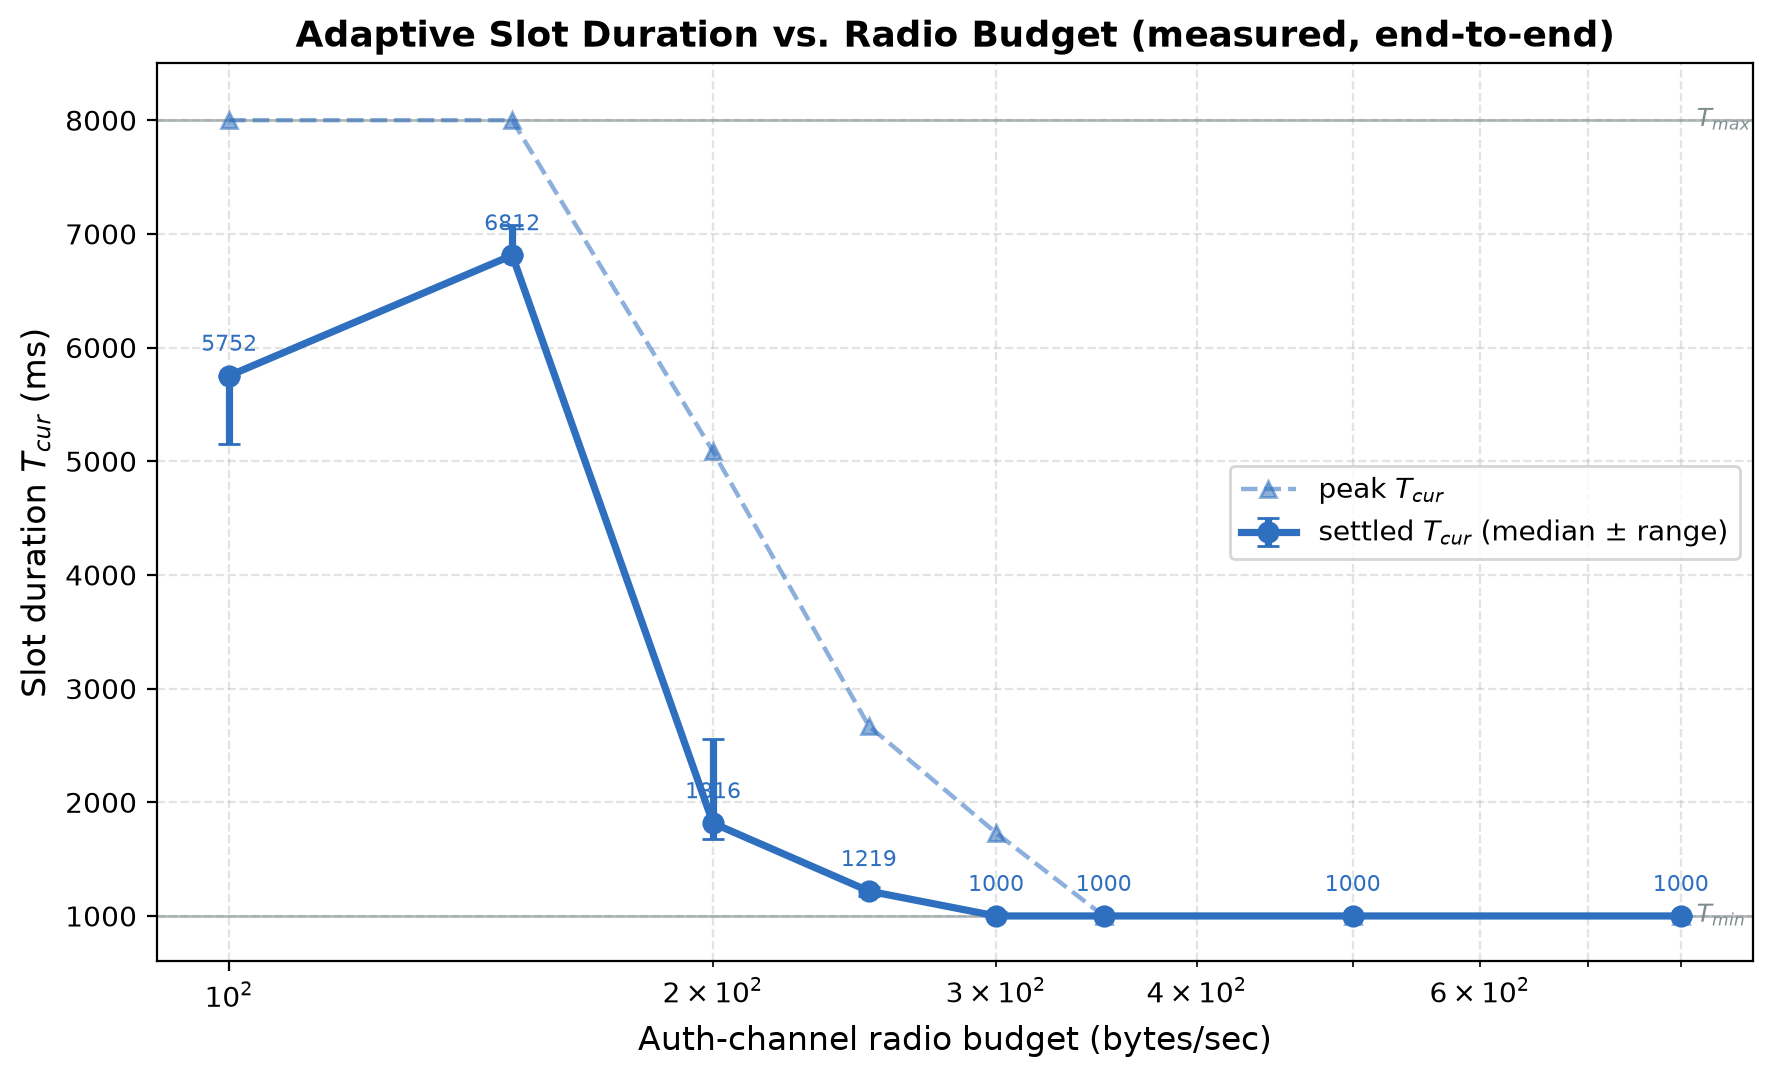
\includegraphics[width=\columnwidth]{figures/fig1_slot_vs_bandwidth.png}
\caption{Adaptive slot duration versus authentication-channel radio budget
(measured, end-to-end). The controller rails at $T_{\max}$ when the budget is
starved, sets a graded duration through the transition, and rests at $T_{\min}$
when the budget is ample. Markers are medians of three runs; bars show the
range.}
\label{fig:slot}
\end{figure}

\subsection{The backlog stays bounded}
Figure~\ref{fig:backlog} plots the disclosure backlog. For every budget at which
authentication is viable the backlog remains a small multiple of the controller
target ($Q_{\text{cap}}/2 = 4$) and well under the device buffer: the loop caps
the queue instead of letting it grow without bound. Only at the starved end
($B=100$\,B/s) does the backlog climb to $14$--$23$ objects---beyond
$Q_{\text{cap}}$---because no slot length can balance production and drainage
there. That point marks the protocol's stability boundary: to its right the
queue is controlled, to its left it overflows.

\begin{figure}[t]
\centering
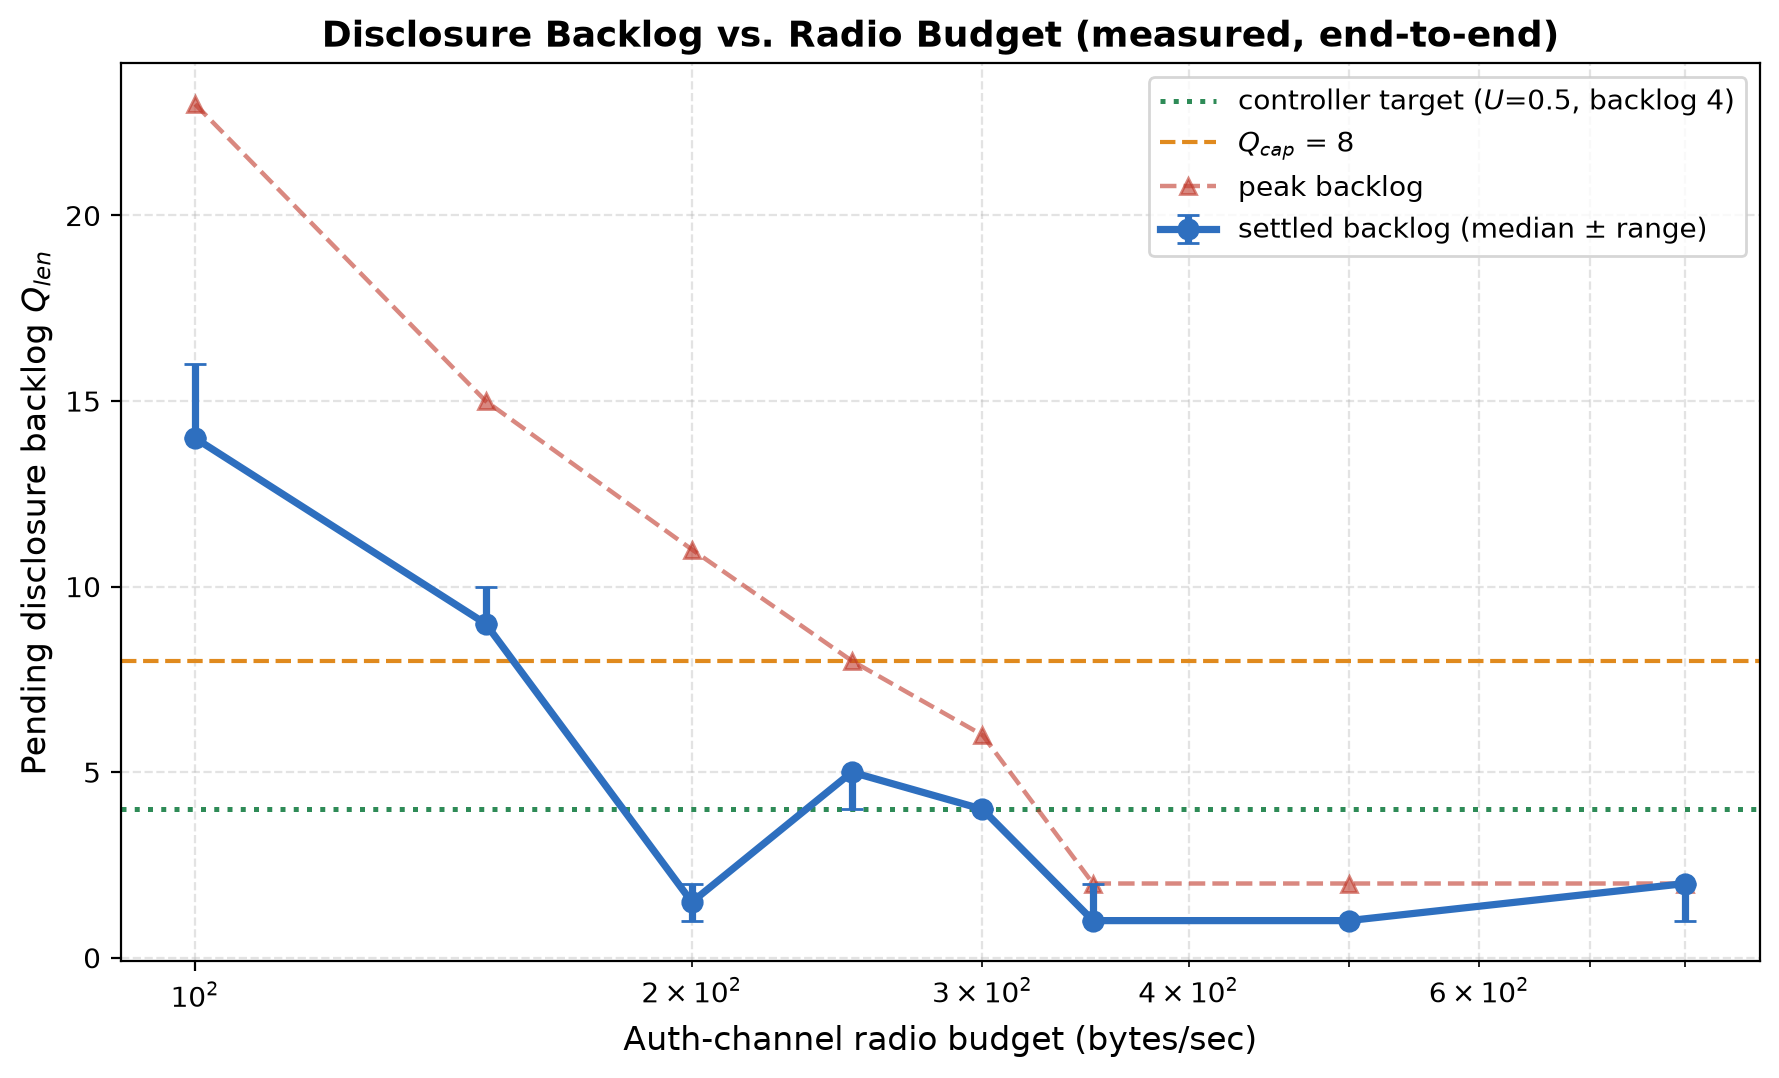
\includegraphics[width=\columnwidth]{figures/fig2_backlog_vs_bandwidth.png}
\caption{Pending-disclosure backlog versus radio budget. The backlog is held
near the controller target across the viable range and blows past $Q_{\text{cap}}$
only at the starved $100$\,B/s point, where even $T_{\max}$ cannot drain it.}
\label{fig:backlog}
\end{figure}

\subsection{Authentication survives to a budget floor}
Figure~\ref{fig:verif} reports receiver outcomes. Above the stability boundary,
verification is healthy (hundreds of messages per run at $500$--$800$\,B/s). As
the budget tightens through the transition the verified count declines but
remains positive, and at the starved $100$\,B/s point it collapses to zero: the
authentication path is so throttled that disclosures cannot reach the receiver
within its timing window, which is precisely the permanent-loss failure the fixed
timer cannot avoid. The premature-rejection count is essentially zero everywhere
except a single spike at $350$\,B/s; as explained in Section~\ref{sec:discussion}
this is a timing artifact of the prototype's slot counter at the $T_{\min}$ knee,
not a forgery.

\begin{figure}[t]
\centering
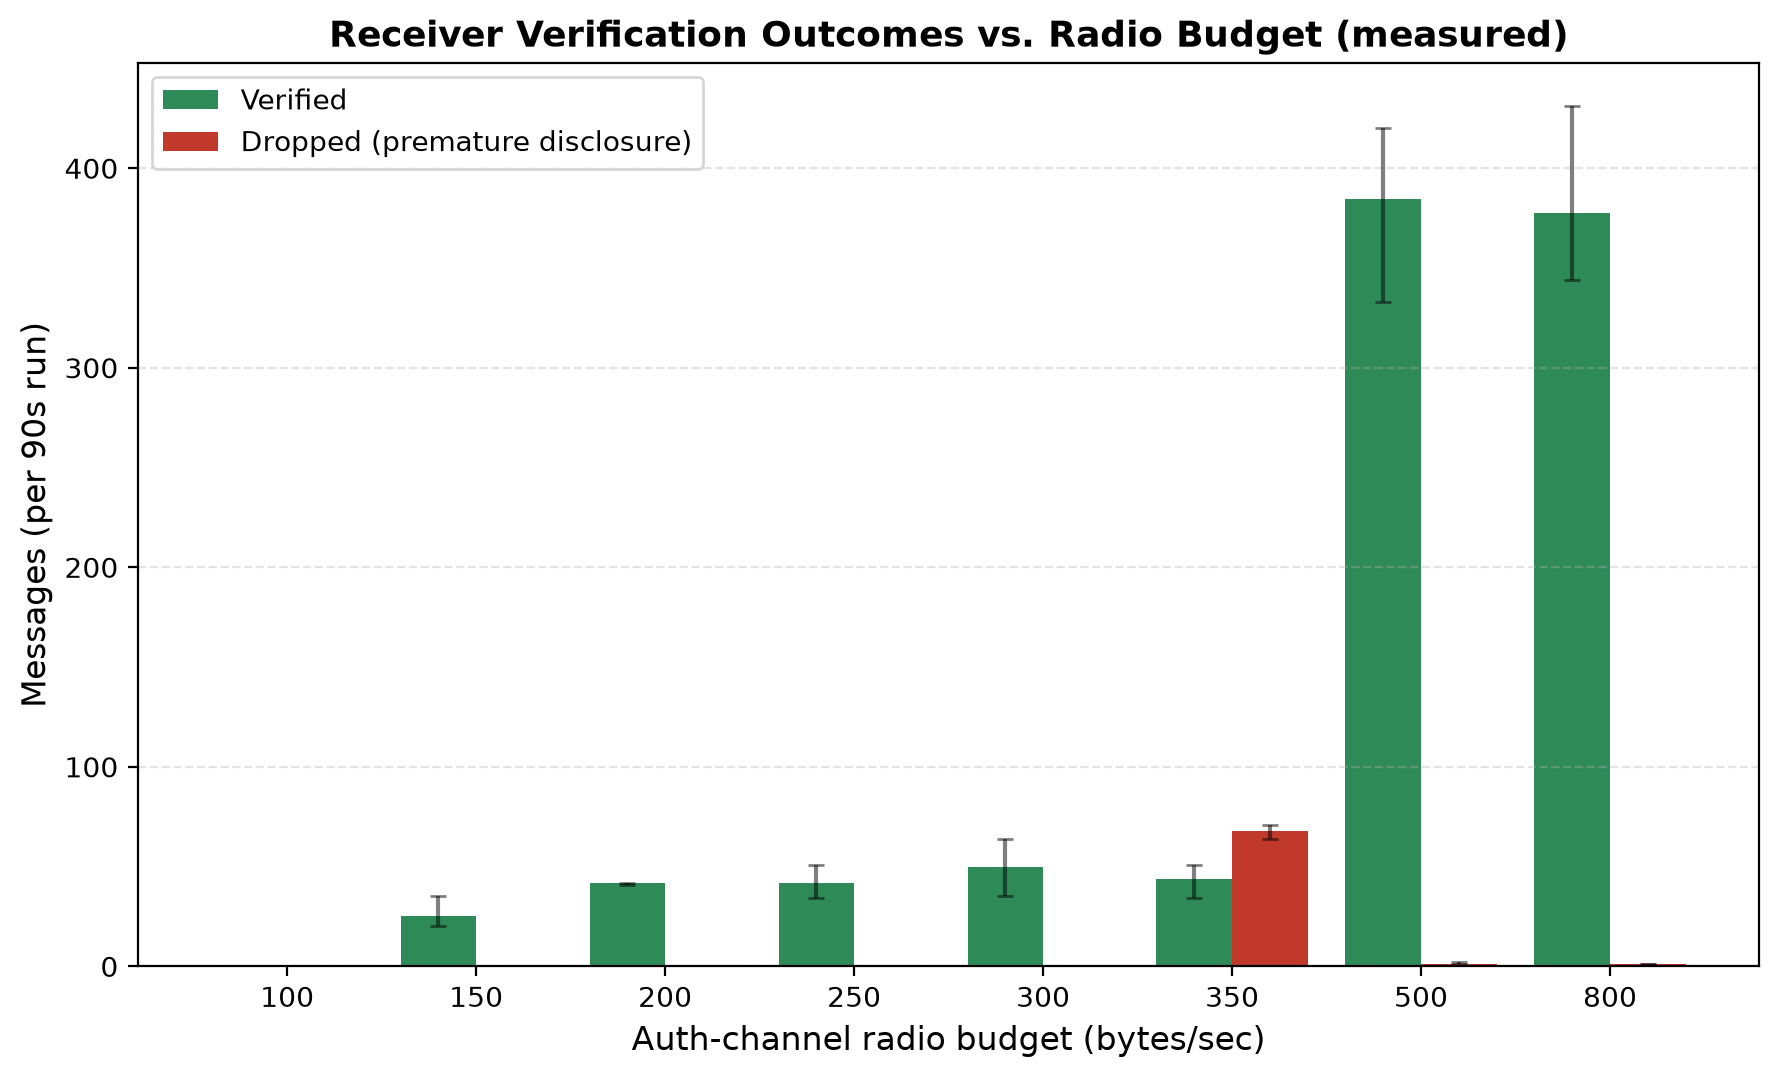
\includegraphics[width=\columnwidth]{figures/fig3_verification_outcomes.png}
\caption{Receiver verification outcomes versus radio budget. Verified messages
are plentiful when the budget is ample, decline through the transition, and
vanish at the starved end; premature rejections are negligible except for one
prototype timing artifact at $350$\,B/s.}
\label{fig:verif}
\end{figure}

\subsection{The control loop, over time}
Figure~\ref{fig:step} shows a single run in the transition regime as a time
series. The backlog and the slot duration trace anti-phase waves: the backlog
rises above the target, the controller raises $T_i$ a few slots later, the longer
slot drains the backlog, $T_i$ then decays, and the cycle repeats. This is the
closed loop in action---the backlog is the cause and the slot duration is the
response, with the expected controller lag. The bounded proportional step, plus
the discrete jumps in Bloom-filter size, make the system limit-cycle around the
target rather than settle to a fixed point, which is why we report robust
steady-state statistics rather than a single terminal value.

\begin{figure}[t]
\centering
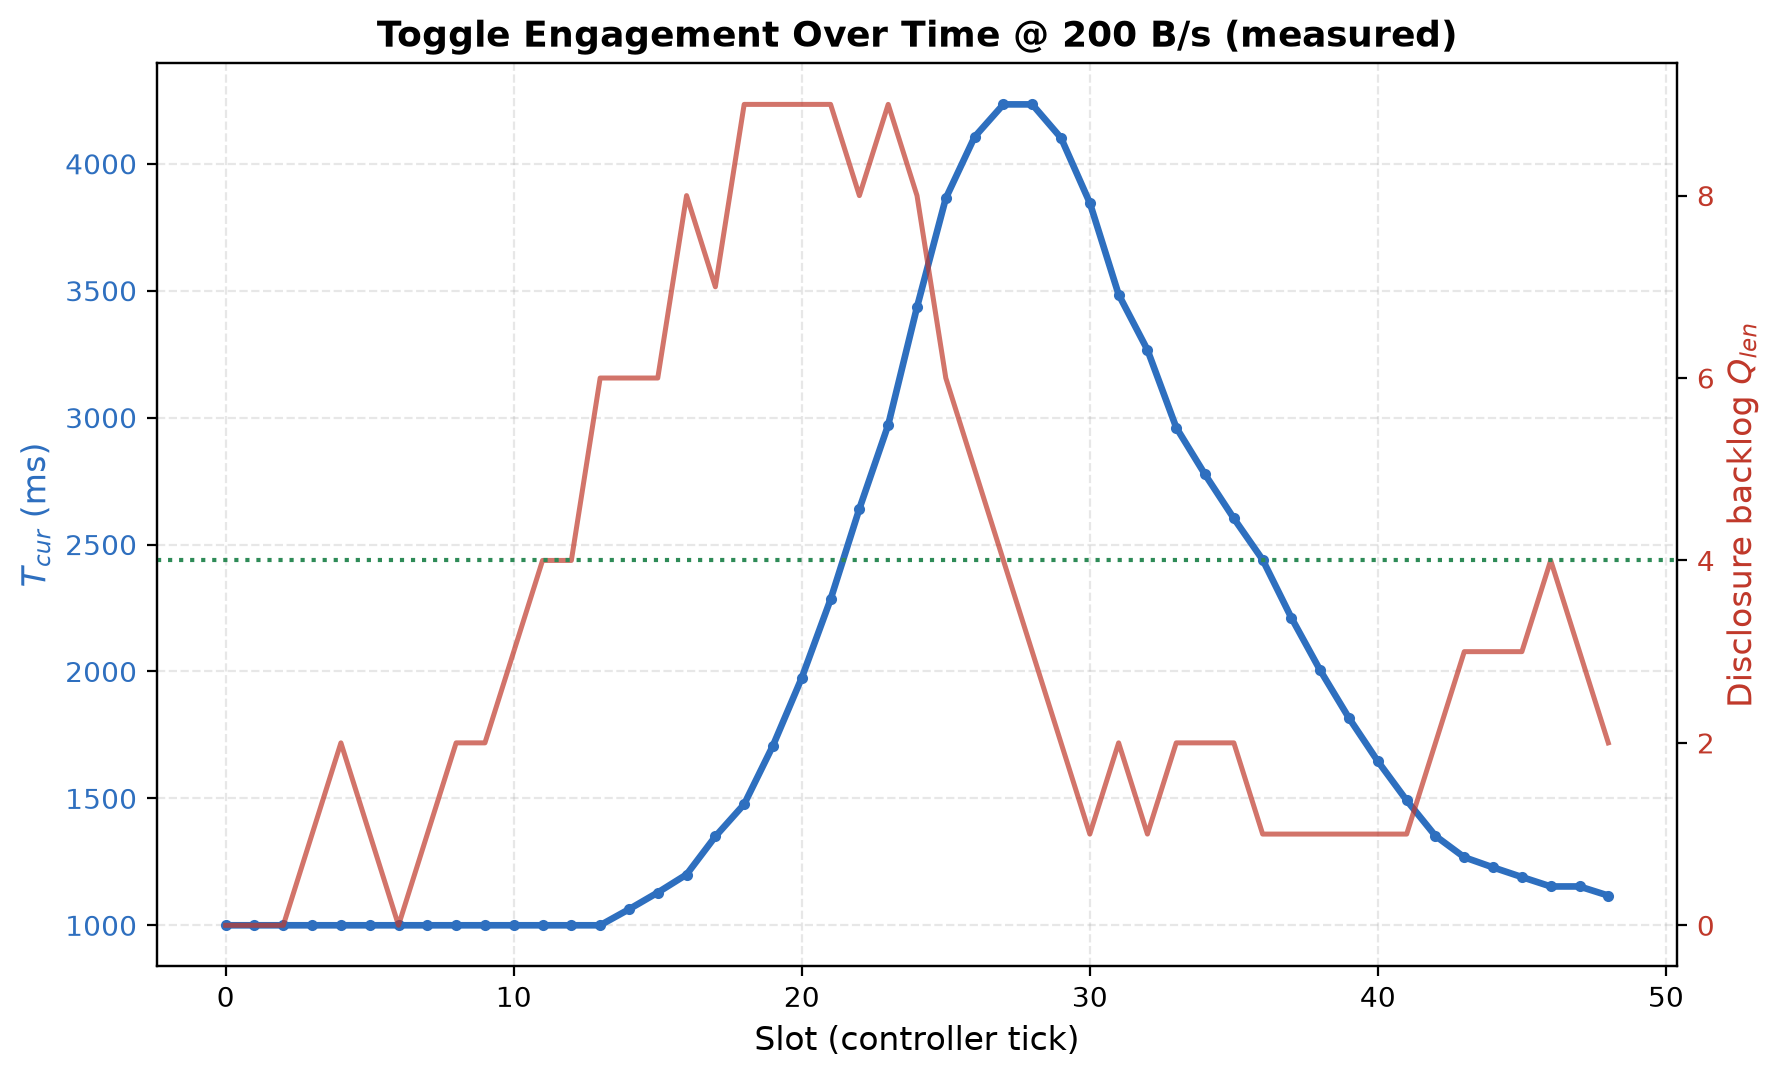
\includegraphics[width=\columnwidth]{figures/fig4_step_timeseries.png}
\caption{Toggle engagement over time in the transition regime. Backlog (right
axis) leads; slot duration (left axis) follows. The dotted line marks the
controller target of four outstanding objects.}
\label{fig:step}
\end{figure}

\subsection{Summary}
Taken together, the figures substantiate the design claim end-to-end: the slot
duration follows the authentication bottleneck, the disclosure backlog stays
bounded across the viable range, and authentication remains alive until a hard
budget floor at which the queue overflows and, as the static protocol also would,
verification fails. The adaptive sender therefore extends the range of radio
conditions over which continuous authentication is preserved, and pays for it
only with additional latency when the channel is genuinely scarce.

\section{Discussion and Limitations}
\label{sec:discussion}
We report the prototype honestly; several caveats bound the strength of the
claims and point at the next steps.

\textbf{Slot-counter timing.} The disclosure worker in the current build advances
the slot counter through a second timer instance in addition to the main slot
loop, so the counter progresses at roughly twice the intended rate and the
effective wall-clock disclosure hold is about half of $d$ slots. Near the
$T_{\min}$ knee this releases keys slightly early relative to the receiver's
security-condition threshold and produces the isolated premature-rejection spike
at $350$\,B/s. The fix---having the worker poll the shared slot counter instead of
opening its own timer---is mechanical and would tighten the transition band; we
report the results with the artifact present and flag it as such.

\textbf{Finite-run steady state.} At the lowest budgets the slot is several
seconds long, so a $90$\,s run contains only a handful of control decisions and
the slot is still climbing toward the ceiling when the run ends. The steady-state
statistic there is therefore conservative; the peak statistic (which reaches
$T_{\max}$) better represents the operating point, and longer runs would close the
gap.

\textbf{Single node over loopback.} Sender and receiver are one process
communicating over the loopback datagram channel. This exercises the full
sender-side controller and the receiver-side checks but does not model
independent clocks, multi-hop delay, or a population of receivers; a multi-node
testbed is the natural next step.

\textbf{Bloom-filter growth.} Because the batch, and hence the Bloom filter,
grows with the slot duration, the per-second authentication byte rate has a
floor set by the message rate. This floor is what creates the hard stability
boundary at the starved end; it is a genuine property of the protocol, not of the
measurement, and should be stated as the limit of what any slot policy can
achieve.

\textbf{Scope of the security argument.} We rely on the security of the
underlying TESLA construction and on the tamper-evidence of the on-chain bounds,
and we do not present a machine-checked timing proof or an adversarial evaluation
of a timing-manipulation attacker. Establishing a receiver-enforced real-time
bound from the on-chain $T_{\max}$, and proving the resulting timing safety, is
deferred to future work.

\section{Related Work}
\label{sec:related}
TESLA~\cite{tesla} and $\mu$TESLA~\cite{spins} established delayed-disclosure
broadcast authentication for wired and sensor settings; the latter targets
resource-constrained motes but assumes periodic resynchronization. Inf-TESLA++
~\cite{inftesla} anchors hash-chain commitments on a blockchain to sustain
authentication across finite chains without sender-assisted resynchronization,
and adds the probabilistic Bloom-filter mode we build on. All of these run a
fixed disclosure schedule. Classical congestion control such as
AIMD~\cite{aimd} assumes per-flow feedback and is unsuitable for one-way,
time-triggered broadcast, where the sender receives no acknowledgements; our
controller instead closes the loop on a purely local signal, the sender's own
disclosure backlog. The bounded proportional update is inspired by the EIP-1559
transaction-fee mechanism~\cite{eip1559}, which likewise steers a quantity toward
a target utilization with a clamped multiplicative step. To our knowledge, making
the TESLA slot duration a closed-loop function of disclosure-queue pressure, with
on-chain duration bounds, is new.

\section{Conclusion and Future Work}
\label{sec:conclusion}
We turned the fixed slot timer of blockchain-anchored, delayed-disclosure
broadcast authentication into a controlled variable. A one-line proportional
rule, reading only the sender's pending-disclosure backlog and clamped to
immutable on-chain bounds, lets the sender stretch its slot under authentication-
channel pressure and shrink it back when the pressure clears, at the cost of a
few arithmetic operations and no extra messages. Running the full
stack---blockchain, owner, and RCD---and sweeping the authentication-channel
radio budget, we measured the controller tracking the bottleneck: the slot rises
to its ceiling as the budget starves, the disclosure backlog stays bounded across
the viable range, and authentication survives down to a hard budget floor set by
the protocol's own batching. Future work will fix the prototype's slot-counter
timing, extend the evaluation to an independent multi-node testbed, add a direct
comparison against fixed-slot baselines across the same budget sweep, and develop
a receiver-enforced real-time bound with a formal timing-safety argument.

\begin{thebibliography}{00}
\bibitem{tesla} A.~Perrig, R.~Canetti, J.~D.~Tygar, and D.~Song, ``The TESLA
broadcast authentication protocol,'' \emph{RSA CryptoBytes}, vol.~5, no.~2,
pp.~2--13, 2002.
\bibitem{spins} A.~Perrig, R.~Szewczyk, J.~D.~Tygar, V.~Wen, and D.~E.~Culler,
``SPINS: Security protocols for sensor networks,'' \emph{Wireless Networks},
vol.~8, no.~5, pp.~521--534, 2002.
\bibitem{inftesla} M.~R.~Dorsala, C.~L.~Nishitha, P.~Sathwik, G.~Srilekha, and
M.~K.~Morampudi, ``Inf-TESLA++: A blockchain-assisted continuous authentication
protocol for broadcast communication in resource-constrained devices,''
Indian Institute of Information Technology Sri City, Chittoor, India.
\bibitem{bloom} B.~H.~Bloom, ``Space/time trade-offs in hash coding with
allowable errors,'' \emph{Communications of the ACM}, vol.~13, no.~7,
pp.~422--426, 1970.
\bibitem{dolevyao} D.~Dolev and A.~C.~Yao, ``On the security of public key
protocols,'' \emph{IEEE Transactions on Information Theory}, vol.~29, no.~2,
pp.~198--208, 1983.
\bibitem{eip1559} T.~Roughgarden, ``Transaction fee mechanism design for the
Ethereum blockchain: An economic analysis of EIP-1559,'' arXiv:2012.00854, 2020.
\bibitem{aimd} D.-M.~Chiu and R.~Jain, ``Analysis of the increase and decrease
algorithms for congestion avoidance in computer networks,'' \emph{Computer
Networks and ISDN Systems}, vol.~17, no.~1, pp.~1--14, 1989.
\end{thebibliography}

\end{document}
